% !TEX root =  ../main_manuscript.tex 
\subsection{Statistical Model}
Modeling an AS dataset such as PRIAS, posed certain challenges. First, PSA was measured longitudinally, and over follow-up time, it did not always increase linearly. Also, PSA was available only until a patient observed upgrading. Hence, we need to accommodate the within-patient correlation for PSA, the association between the Gleason grades and PSA profiles of a patient, and handle missing PSA measurements after a patient experienced upgrading. Second, since the PRIAS biopsy schedule uses PSA, a patient's observed time of upgrading was also dependent on their PSA. Thus, the effect of PSA on the upgrading-risk need to be adjusted for the effect of PSA on the biopsy schedule. Third, many patients obtained treatment and watchful waiting before observing upgrading. Since we considered events other than upgrading as censoring, the model needs to account for patients' reasons for treatment or watchful waiting (e.g., age, treatment based on observed data). A model that handles these challenges in a statistically sound manner is the joint model for time-to-event and longitudinal data~\citep{tomer2019,coley2017prediction,rizopoulos2012joint}. 

Our joint model consisted of two sub-models. Namely, a linear mixed-effects sub-model~\citep{laird1982random} for longitudinally measured PSA (log-transformed), and a relative-risk sub-model (similar to the Cox model) for the interval-censored time of upgrading. Patient age was used in both sub-models. Results and timing of the previous negative biopsies were used only in the risk sub-model. To account for PSA fluctuations~\citep{nixon1997biological}, we assumed t-distributed PSA measurement errors. The correlation between PSA measurements of the same patient was established using patient-specific random-effects. We fitted a unique curve to the PSA measurements of each patient (Panel~A, Figure~\ref{fig:jmExplanationPlot_113}). Subsequently, we calculated the mathematical derivative of the patient's fitted PSA profile (Equation~2, Supplementary~A), to obtain his follow-up time specific instantaneous PSA velocity (Panel~B, Figure~\ref{fig:jmExplanationPlot_113}). This instantaneous velocity is a stronger predictor of upgrading than the widely used average PSA velocity~\citep{cooperberg2018refined}. We modeled the impact of PSA on upgrading-risk by employing fitted PSA value and instantaneous velocity as predictors in the risk sub-model (Panel~C, Figure~\ref{fig:jmExplanationPlot_113}). We adjusted the effect of PSA on upgrading-risk for the PSA dependent PRIAS biopsy schedule by estimating parameters using a full likelihood method (proof in Supplementary~A). This approach also accommodates watchful waiting and treatment protocols that are also based on patient data. Specifically, the parameters of our two sub-models were estimated jointly under the Bayesian paradigm (Supplementary~A) using the R package \textbf{JMbayes}~\citep{rizopoulosJMbayes}.

\begin{figure}
\centerline{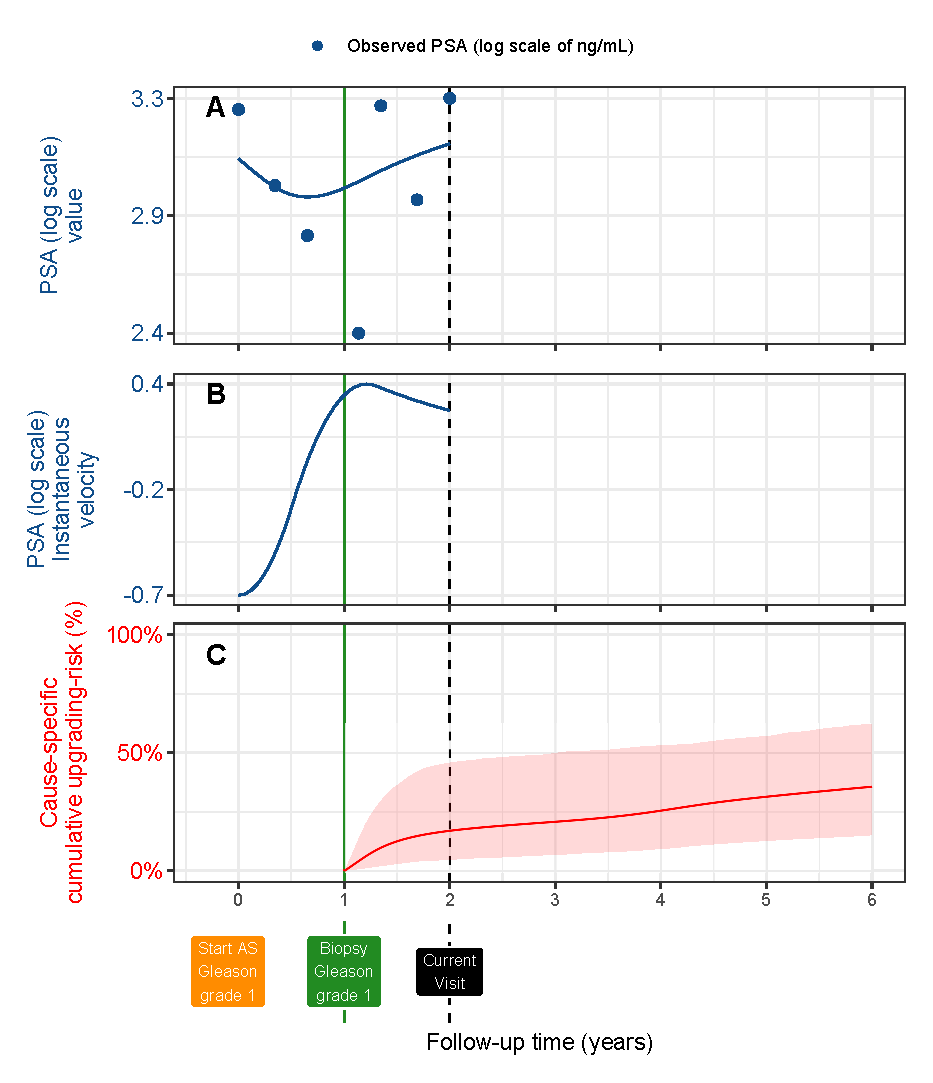
\includegraphics[width=\columnwidth]{images/jmExplanationPlot_113.eps}}
\caption{\textbf{Illustration of the joint model on a real PRIAS patient}. \textbf{Panel~A:} Observed PSA (blue dots) and fitted PSA (solid blue line), log-transformed from ng/mL. \textbf{Panel~B:} Estimated instantaneous velocity of PSA (log-transformed). \textbf{Panel~C}: Predicted cause-specific cumulative upgrading-risk (95\% credible interval shaded). Upgrading is defined as an increase in the Gleason grade group from group~1~\citep{epsteinGG2014} to 2 or higher. This upgrading-risk is calculated starting from the time of the latest negative biopsy (vertical green line at year one of follow-up). The joint model estimated it by combining the fitted PSA (log scale) value and instantaneous velocity, and time of the latest negative biopsy. Black dashed line at year two denotes the time of current visit.}
\label{fig:jmExplanationPlot_113}
\end{figure}

\subsection{Risk Prediction and Model Validation}
Our model provides predictions for upgrading-risk over the entire future follow-up period of a patient (Panel~C, Figure~\ref{fig:jmExplanationPlot_113}). However, we recommend using predictions only after year one. This is because most AS programs recommend a confirmatory biopsy at year one, especially to detect patients who may be misdiagnosed as low-grade at inclusion in AS. The model also automatically updates risk-predictions over follow-up as more patient data becomes available (Figure~5, Supplementary~B). We validated our model internally in the PRIAS cohort, and externally in the largest six GAP3 database cohorts. We employed calibration plots~\citep{royston2013external,steyerberg2010assessing} and follow-up \textit{time-dependent} mean absolute risk prediction error or MAPE~\citep{rizopoulos2017dynamic} to graphically and quantitatively evaluate our model's risk prediction accuracy, respectively. We assessed our model's ability to discriminate between patients who experience/do not experience upgrading via the time-dependent area under the receiver operating characteristic curve or AUC~\citep{rizopoulos2017dynamic}. 

The aforementioned \textit{time-dependent} AUC and MAPE~\citep{rizopoulos2017dynamic} are temporal extensions of their standard versions~\citep{steyerberg2010assessing} in a longitudinal setting. Specifically, at every six months of follow-up, we calculated a unique AUC and MAPE for predicting upgrading-risk in the subsequent one year (Supplementary~B.1). For emulating a realistic situation, we calculated the AUC and MAPE at each follow-up using only the validation data available until that follow-up. Last, to resolve any potential model miscalibration in validation cohorts, we aimed to recalibrate our model's baseline hazard of upgrading (Supplementary~B.1), individually for each cohort.